% Basic stuff
\documentclass[a4paper,10pt]{article}
\usepackage[nswissgerman]{babel}
\usepackage{scrextend}

% 3 column landscape layout with fewer margins
\usepackage[landscape, left=0.75cm, top=1cm, right=0.75cm, bottom=1.5cm, footskip=15pt]{geometry}
\usepackage{flowfram}
\usepackage{multicol}
\ffvadjustfalse
\setlength{\columnsep}{1cm}
\Ncolumn{3}

% define nice looking boxes
\usepackage[many]{tcolorbox}

\changefontsizes[9pt]{9pt}

% a base set, that is then customised
\tcbset {
  base/.style={
    boxrule=0mm,
    leftrule=1mm,
    left=1.75mm,
    arc=0mm, 
    fonttitle=\bfseries, 
    colbacktitle=black!10!white, 
    coltitle=black, 
    toptitle=0.75mm, 
    bottomtitle=0.25mm,
    title={#1}
  }
}

\definecolor{brandblue}{rgb}{0.34, 0.7, 1}
\newtcolorbox{mainbox}[1]{
  colframe=brandblue, 
  base={#1}
}

\newtcolorbox{subbox}[1]{
  colframe=black!20!white,
  base={#1}
}

% Mathematical typesetting & symbols
\usepackage{amsthm, mathtools, amssymb} 
\usepackage{marvosym, wasysym}
\usepackage{derivative}
\allowdisplaybreaks

% Tables
\usepackage{tabularx, multirow}
\usepackage{booktabs}

% Make enumerations more compact
\usepackage{enumitem}
\setitemize{itemsep=0.5pt}
\setenumerate{itemsep=0.75pt}

% To include sketches & PDFs
\usepackage{graphicx}

% For hyperlinks
\usepackage{hyperref}
\hypersetup{
  colorlinks=true
}

% Metadata
\title{Cheatsheet Analysis 2}
\author{Thomas Gassmann}
\date{January 2023}

% Math helper stuff
\def\limn{\lim_{n\to \infty}}
\def\limxo{\lim_{x\to 0}}
\def\limxi{\lim_{x\to\infty}}
\def\limxn{\lim_{x\to-\infty}}
\def\sumk{\sum_{k=1}^\infty}
\def\sumn{\sum_{n=0}^\infty}
\def\R{\mathbb{R}}
\def\C{\mathbb{C}}
\def\Q{\mathbb{Q}}
\def\N{\mathbb{N}}
\def\X{\mathcal{X}}
\def\dx{\mathop{dx}}
\def\dy{\mathop{dy}}

\DeclareMathOperator{\vol}{\text{vol}}
\DeclareMathOperator{\interior}{\text{int}}

\begin{document}

% ! TeX root = ...

\begin{center}
    Lizenziert unter CC BY-SA 4.0. Für Urheber, Quellen und Lizenzinformationen, siehe:\\
    \href{https://github.com/thomasgassmann/eth-summaries}{github.com/thomasgassmann/eth-summaries}
\end{center}


\section{Differentialgleichungen}
\begin{mainbox}{Definition lineare DGL}
  Eine gewöhnliche lineare Differentialgleichung $n$-ter Ordnung ist eine Gleichung, welche Ableitungen enthält. Sie hat die Form \[a_n y^{(n)} + a_{n-1} y^{(n-1)} + \cdots + a_0y = b(x)\]
  wobei die Koeffizienten \(a_0(x), \ldots, a_{n}(x)\) stetige komplexe Funktionen auf \(I \subseteq \R\) sind. Wenn \(b(x) = 0\) gilt, ist die DGL homogen.
\end{mainbox}

\(S_0\) ist das Set der Lösungen zu einer homogenen DGL und bidlet einen Vektorraum der Dimension $n$. Linearkombinationen von Lösungen der DGL sind also auch wieder Lösungen.\\

Für jede Anfangsbedingung der Form

$$y(x_0) = y_0, y'(x_0) = y_1, \cdots, y^{k-1}(x_0) = y_{k-1}$$

gibt es eine eindeutige Lösung $y(x)$, welche die Anfangsbedingungen erfüllt.\\

Die \textbf{allgemeine Lösung} einer DGL setzt sich dann aus einer homogenen Lösung und einer speziellen Lösung zusammen ($f(x) = f_h(x) + f_p(x)$).

\subsubsection*{Lineare DGL erkennen}
\begin{itemize}
  \item alle Koeffizienten sind stetige Funktionen
  \item keine Produkte von $y$ oder deren Ableitungen
  \item keine Potenzen von $y$ oder deren Ableitungen
  \item keine Funktionen von $y$ oder deren Ableitungen
\end{itemize}

\subsubsection*{Substitution}

Manchmal ist es hilfreich $y(x)$ durch eine Funktion $h(x) = y(g(x))$ zu ersetzen. Betrachten wir die DGL $x^2 y''(x) - 3xy'(x) + 5y(x) = 0$. Wählen wir $h(t) = y(e^t)$ lässt sich die DGL mit konstanten Koeffizienten lösen (denn $x = e^t$).

\subsection{Separierbare DGL}

Eine Separierbare ODE erster Ordnung hat die Form $y' = b(x) g(y)$. Wir können diese dann nach $y$ und $x$ separieren und erhalten dann $\frac{y'}{g(y)} = b(x)$. Durch integrieren auf beiden Seiten und einer Substitution von $y$ erhalten wir dann:

$$\int \frac{1}{g(y)} \dy = \int b(x) \dx$$

\subsection{Lineare DGL erster Ordnung}
Wir betrachten DGL der Form \[y' + a(x)y = b(x)\]
\begin{enumerate}
  \item (Homogene Lösung) 
  \begin{align*}
    y' + a(x)y &= 0\\
    \frac{y'}{y} &= -a(x)\\
    \ln(y) &= -A(x)+C\\
    y &= e^{-A(x)+C} = z \cdot e^{-A(x)}\quad z \in \C
  \end{align*}\\
  Haben wir ein Anfangswertproblem der Form $f(x_0) = y_0$ so erhalten wir für $f_h(x) = y_0 e^{A(x_0) - A(x)}$.
  \item (partikuläre Lösung) Verwende entweder ``Variation der Konstanten'' oder ``Fundiertes Raten''.
\end{enumerate}
\subsection{Variation der Konstanten}
Wir nehmen an, dass die partikuläre Lösung die homogene Lösung imitiert. Sei \(f_p = z(x)e^{-A(x)}\) für eine Funktion \(z: I \to \C\). Dann ist \(z'(x) = b(x) e^{A(x)}\) (einsetzen in DGL $y' + a(x)y = b(x)$) und somit \[z(x) = \int b(x) e^{A(x)} \mathop{dx}\] Daraus erhalten wir \[f_p = e^{-A(x)} \int b(x) e^{A(x)} \mathop{dx}\]

\subsection{Fundiertes Raten}

Wir nehmen an, dass die partikuläre Lösung $b$ imitiert. Wenn $b(x)$ von einer bestimmten Form ist, versuchen wir folgende $f_p$, wobei wir unseren Versuch in die DGL einsetzen, was uns dann ein Gleichungssystem für die Konstanten gibt:

\begin{center}
  \renewcommand*{\arraystretch}{1.5} 
  \begin{tabular}{cc}
    \toprule
    $\mathbf{b(x)}$ & \textbf{Raten} \\ 
    \midrule
    $P_n(x) \cdot e^{\alpha x}$ & $R_n(x) \cdot e^{\alpha x}$\\
    \hline
    \begin{tabular}{@{}c@{}}$P_n(x) \sin(\beta x)\text{ or }$ \\ $P_n(x) \cos(\beta x)$\end{tabular} & $R_n(x) \sin(\beta x) + S_n(x) \cos(\beta x)$\\
    \hline
    \begin{tabular}{@{}c@{}}$P_n(x) e^{\alpha x} \sin(\beta x)\text{ or }$ \\ $P_n(x) e^{\alpha x} \cos(\beta x)$\end{tabular} & $e^{\alpha x}\left( R_n(x) \sin(\beta x) + S_n(x) \cos(\beta x) \right)$\\
    \bottomrule
  \end{tabular}
\end{center}

\(P_n, R_n \) und \(S_n\) sind Polynome von Grad $n$ in \(x\). 

\begin{enumerate}
  \item Wenn \(b(x)\) eine Linearkombination der Basisfunktionen ist, dann versuche eine Linearkombination. Partikuläre Lösungen können auch separat gefunden werden und danach addiert werden.
  \item \textbf{Für DGL mit konstanten Koeffizienten:} Falls $\lambda = \alpha + i \beta$ eine Wurzel des charakteristischen Polynoms mit Vielfachheit $m$ ist, dann multiplizieren wir die geratene Lösung mit $x^m$.
\end{enumerate}

\subsection{Lineare DGL mit konstanten Koeffizienten}
Wir betrachten DGL der Form
\[a_k y^{(k)} + a_{k-1} y^{(k-1)} + \ldots + a_1 y' + a_0 y = b(x)\]
Wir suchen eine homogene Lösung der Form \(e^{\lambda x}\). Jetzt können wir das charakteristische Polynom lösen:
\begin{align*}
  P(\lambda) = e^{\lambda x} \left(a_k \lambda^k + a_{k-1}\lambda^{k-1} + \ldots + a_0\right) = 0 \\ 
  \implies 0 = a_k \lambda^k + a_{k-1}\lambda^{k-1} + \ldots+ a_0
\end{align*}

Die Nullstellen von \(P(\lambda)\) sind Eigenwerte \(\lambda_i\), mit dazugehöriger Multiplizität \(m_i\). Nun spannen die folgenden Funktionen den Raum der Lösungen \(S_0\) auf:
\begin{align*}
  & f_{i,r} : x \to x^r e^{\lambda_i x} & 0 \leq r < m_i &
\end{align*}

Falls \(\lambda = \beta + \gamma i\) eine komplexe Nullstelle von einem Polynom mit reellen Koeffizienten \(P(\lambda)\) ist, so ist auch 
\(\bar{\lambda} = \beta - \gamma i\) eine Nullstelle. Daher sind \(f_1 = e^{\lambda x}\) und \(f_2 = e^{\bar{\lambda} x}\) Lösungen und können durch eine Linearkombination von \(\tilde{f_1} = e^{\beta x} \cos(\gamma x)\) und \(\tilde{f_2} = e^{\beta x} \sin(\gamma x)\) ersetzt werden.

Falls \(a_k y^{(k)} + a_{k-1}y^{(k-1)} + \dots + a_0 y = 0\) reelle Koeffizienten hat, so führt jedes Paar von komplex konjugierten Nullstellen $\beta_j \pm \gamma_j i$ mit Multiplizität $m_j$ zu einer Lösung
\[x^l e^{\beta_j x} \Big( c_0 \cos(\gamma_j x) + c_1 \sin(\gamma_j x) \Big) \quad \text{für }0 \leq l < m_j\]

Um eine partikuläre Lösung zu finden, können wir wieder fundiertes Raten oder Variation der Konstanten verwenden. 
Variation der Konstanten funktioniert wie folgt (hier 2D):

\begin{enumerate}[label=(\arabic*)]
  \item Nimm an, dass die homogene Lösung \(f = z_1 f_1 + z_2 f_2\) ist
  \item Versuche nun \(f_p = z_1(x) f_1 + z_2(x) f_2\)
  \item Löse das folgende System
  \begin{align*}
    z_1'(x) f_1 + z_2'(x) f_2 &= 0\\
    z_1'(x) f_1' + z_2'(x) f_2' &= b(x)\\
  \end{align*}
  Hier gehen wir wie folgt vor:
  \begin{align*}
    W &= f_1 f_2' - f_2 f_1' \neq 0\\
    \Rightarrow z_1' &= \frac{-f_2 b}{W} \; , z_2' = \frac{-f_1 b}{W}\\
    \Rightarrow f_p &= -f_1 \int \frac{f_2 b}{W} dt + f_2 \int \frac{f_1 b}{W} dt
  \end{align*}
\end{enumerate}

\section{Ableitungen in \texorpdfstring{\(\R^n\)}{Rⁿ}}
\begin{subbox}{Monom}
  Ein Monom vom Grad \(e\) ist
  \begin{align*}
    (x_1, \ldots, x_n) \mapsto x_1^{d_1}\cdot \ldots \cdot x_n^{d_n} \\
    e = d_1 + \ldots + d_n 
  \end{align*}
  \(\to\) ein Polynom, das nur aus einem Glied besteht.
\end{subbox}
\begin{mainbox}{Polynom}
  Ein Polynom mit \(n\) Variablen vom Grad \(d\) ist eine endliche Summe von Monomen mit Grad \(e \le d\).
\end{mainbox}

\subsection{Konvergenz}
\begin{enumerate}
  \item Skalarprodukt: \(\left< x,y\right> = \sum_{i=0} x_i \cdot y_i\)
  \item Euklidische Norm: \(||x|| := \sqrt{x_2^1 + \cdots + x_n^2}\) mit den folgenden Eigenschaften:
  \begin{enumerate}
    \item \(||x|| \ge 0, ||x|| = 0 \iff x = 0\)
    \item \(||\lambda x|| = |\lambda| \cdot ||x||, \forall \lambda \in \R\)
    \item \(||x+y|| \le ||x|| + ||y||\)
    \item \(|\left<x,y\right>| \le ||x|| \cdot ||y||\)
  \end{enumerate}
\end{enumerate}

\begin{mainbox}{Definition Konvergenz}
  Sei \((x_k)_{k \in \mathbb{N}}, x_k \in \R^n\). Die folgenden Definitionen sind für \(\lim_{k\to\infty}x_k = y\) äquivalent:
  \begin{enumerate}
    \item \(\forall \epsilon > 0 \exists N \ge 1\) so dass \(\forall k \ge N \ ||x_k - y|| < \epsilon\).
    \item Für jedes \(i, 1 \le i \le n\) konvergiert die Folge \((x_{k,i})_k\) von reellen Zahlen nach \(y_i\).
    \item Die Folge der reellen Zahlen \(||x_k - y||\) konvergiert nach \(0\).
  \end{enumerate}
\end{mainbox}
\subsection{Stetigkeit}
Sei \(f: \X \subseteq \R^n \to \R^m\)  und \(x_0 \in \X\). \(f\) ist stetig in \(x_0\), falls eine der folgenden Bedingungen erfüllt ist:
\begin{enumerate}
  \item \(\forall \epsilon > 0 \exists \delta > 0\) so dass \(\forall x \in \X \) \(||x - x_0|| < \delta \implies ||f(x) - f(x_0)|| < \epsilon\).
  \item Für alle Folgen \((x_k)\) in \(X\) mit \(\lim_{k \to \infty} x_k = x_0\) gilt \(\lim_{k \to \infty} f(x_k) = f(x_0)\).
\end{enumerate}
\(f\) ist stetig in \(\X\) falls \(f\) für jeden Punkt \(x_0 \in \X\) stetig ist. Es gilt:
\begin{enumerate}
  \item \(f(x = x_1, \ldots, x_n) \mapsto (f_1(x),\ldots,f_m(x))\) und \(f_i: \R^n \to \R\) stetig \(\iff \forall i = 1, \ldots, m \ f_i\) stetig.
  \item Lineare Funktionen \(x \mapsto Ax\) sind stetig.
  \item Polynome sind stetig.
  \item Summen + Produkte von stetigen Funktionen sind stetig.
  \item Funktionen unterschiedlicher Variablen sind stetig, falls alle Variablen stetig sind.
  \item Verknüpfungen stetiger Funktionen sind stetig.
\end{enumerate}
\begin{mainbox}{Sandwich-Lemma}
  Wenn \(f, g, h: \R^n \to \R\) Funktionen mit \(f(x) < g(x) < h(x) \forall x \in \R^n\) sind, dann gilt
  \[\lim_{x\to a} f(x) = \lim_{x \to a} h(x) = L \implies \lim_{x\to a} g(x) = L\]
\end{mainbox}
\subsection{Eigenschaften von Mengen}
Eine Menge \(\X \subseteq \R^n \) ist
\begin{itemize}
  \item \textbf{beschränkt}, falls \(\exists R \ge 0, \forall x \in \X: ||x|| \le R\).
  \item \textbf{abgeschlossen}, falls jede Folge \((x_k)_{k\in \N} \subseteq \X\), die in \(\R^n\) konvergiert, zu einem Punkt in \(\X\) konvergiert. Dies kann mit einem Ball visualisiert werden. \\Urbilder von offenen (resp. abgeschlossenen) Mengen sind unter stetigen Abbildungen offen (resp. abgeschlossen). Die Umkehrung ist im Allgemeinen falsch.\\
  Gegenbeispiele: \(\frac{1}{k}, <\).
  \item \textbf{kompakt}, falls sie beschränkt und abgeschlossen ist. Bilder von kompakten Mengen sind unter stetigen Abbildungen kompakt.
  \item \textbf{offen}, falls ihr Komplement \(\R^n \setminus \X\) abgeschlossen ist. Alternativ: für jedes $x_0 \in \X$ gibt es ein $\delta > 0$ so dass $B_\delta(x_0) \subseteq \X$.
  \item \textbf{konvex}, falls \(\forall x, y \in \X: \lambda x + (1 - \lambda)y \in \X\) gilt (die Linie zwischen \(x, y\) ist in \(\X\)).
\end{itemize}

Es gilt dabei:

\begin{itemize}
  \item Falls $\{X_\alpha\}_{\alpha \in I}$ eine Menge von offenen (resp. abgeschlossen) Mengen. Dann ist $\cup_{\alpha \in I} X_\alpha$ offen (respektive $\cap_{\alpha \in I} X_\alpha$ abgeschlossen).
  \item Falls $\{X_\alpha\}_{\alpha \in I}$ eine \textbf{endliche} Menge von offenen (resp. abgeschlossen) Mengen. Dann ist $\cap_{\alpha \in I} X_\alpha$ offen (respektive $\cup_{\alpha \in I} X_\alpha$ abgeschlossen).
  \item Das kartesische Produkt zweier offenen Mengen ist offen.
  \item $\emptyset$ und $\R^n$ sind offen \textbf{und} abgeschlossen.
\end{itemize}

Beispiele:
\begin{itemize}
  \item \((a,b) \subseteq \R\) ist offen.
  \item \(\left[a,b\right) \subseteq \R\) ist weder offen noch abgeschlossen.
  \item \(\R^n\) und \(\varnothing\) sind offen.
  \item \((a_1, b_1) \times (a_2,b_2) \subseteq \R^2\) ist offen.
\end{itemize}

\begin{subbox}{Bolzano-Weierstrass}
  Jede beschränkte Folge in \(\R^n\) hat eine konvergente Teilfolge.
\end{subbox}
\begin{subbox}{Min-Max-Theorem}
  Sei \(\X \subseteq \R^n, \X \ne \varnothing\) eine kompakte Menge und \(f: \X \to \R\) eine stetige Funktion. Dann ist \(f\) beschränkt und ein Maximum \(x^+\)/Minimum \(x^-\)existieren, so dass
  \[f(x^+) = \sup_{x\in \X} f(x) \quad f(x^-) = \inf_{x \in \X} f(x)\]
\end{subbox}
\subsection{Partielle Ableitungen}
Um eine partielle Ableitung von \(f: \X \subseteq \R^n \to \R\) (wobei \(\X\) offen) zu finden, betrachten wir alle Variablen bis auf eine als konstant und leiten nach dieser ab.
\[\pdv{f}{x_{0,j}} = \lim_{h \to 0} \frac{f(x_{0,1}, \ldots, x_{0,j} + h, \ldots, x_{0,n}) - f(x_0)}{h}\]
Für \(f: \R^n \to \R^m, x_0 \in \R^n\) gilt
\begin{align*}
  \pdv{f(x_0)}{x_j} := \begin{pmatrix}
    \pdv*{f_1(x_0)}{x_j}\\
    \vdots\\
    \pdv*{f_m(x_0)}{x_j}\\
  \end{pmatrix}
\end{align*}
Partielle Ableitungen haben folgende Eigenschaften:
\begin{enumerate}
  \item \(\partial_j(f + g) = \partial_j (f) + \partial_j g\)
  \item \(\partial_j(f \cdot g) = \partial_j (f) \cdot g + \partial_j (g) \cdot f\)
  \item \(\partial_j(f / g) = \frac{\partial_j (f) \cdot g - \partial_j (g) \cdot f}{g^2}\) für \(g \ne 0\)
\end{enumerate}
\begin{mainbox}{Jacobi-Matrix}
Sei \(f: \X \subseteq \R^n \to \R^m\) und \(\X\) eine offene Menge. Die Jacobi-Matrix ist eine Matrix mit \(m\) Zeilen und \(n\) Spalten:
\[J_f = \left( \pdv{f_i}{x_j} \right)_{\substack{1 \leq j \leq n \\ 1 \leq i \leq m}}\]
\end{mainbox}
\begin{mainbox}{Gradient}
  Die transponierte Jacobi-Matrix einer Funktion \(f: \X \subseteq \R^n \to \R\) ist ein Spaltenvektor, der mit \(\nabla f\) bezeichnet wird. Die geometrische Interpretation ist ein Vektorfeld, definiert durch \(\nabla f\), welches die Richtung und Magnitude des grössten Wachstums von \(f\) angibt.
\end{mainbox}
\begin{subbox}{Divergenz}
  Die Divergenz einer Funktion \(f\) ist die Spur der Jacobi-Matrix von \(f\). \[\text{div}(f)(x_0) = \text{Tr}(J_f(x_0)) = \sum_{i=0}(J_f)_{i,i}\]
\end{subbox}

Allgemeiner als die partiellen Ableitungen kann man auch die Richtungsableitung definieren. Für $v \in \R^n$ ($\lVert v \rVert = 1$) und $f: \R^n \to \R^m$ ist die Richtungsableitung $D_v f$ definiert als:

$$D_v f(x) = \lim_{h \rightarrow 0} \frac{f(x + hv) - f(x)}{h}$$

 Die Richtungsableitung $D_v f(x)$ existiert, wenn $t \mapsto f(x + hv)$ in $h = 0$ differenzierbar ist. Es gilt $D_v f(x) = D f(x) v$. Für die $k$-te partielle Ableitungen gilt dann $\frac{\partial f}{\partial x_k} = D_{e_k} f$.

\subsubsection*{Landau Notation in der Analysis}

Es gilt $f \in o(h)$ falls:

$$\lim_{h \to 0} \frac{f(h)}{h} = 0$$

In der Analysis betrachtet man die Landau Notation generell für $\lim_{h \to 0}$ statt $\lim_{h \to \infty}$. Es gilt deshalb bspw. $x^5 \in \mathcal{O}(x^4)$.

\subsection{Differenzierbarkeit}
Sei \(f: \X \subseteq \R^n \to \R^m, x_0 \in \X\). \(f\) ist differenzierbar an der Stelle \(x_0\), falls eine lineare Abbildung \(L: \R^n \to \R^m\) (d.h. eine \(m \times n\)-Matrix \(L\)) existiert, so dass \(\forall x_0 + v \in \X\):
\[f(x_0 + v) = f(x_0) + L(v) + R(x_0,v)\]
wobei für den Fehlerterm \(R\) folgendes gilt: 
$$\lim_{v \to 0} \frac{||R(x_0,v)||}{||v||} = 0 \iff R(x_0, v) \in o(||v||)$$

Äquivalent dazu gilt also dass $f$ differenzierbar in $x_0$ ist falls $\lim_{v \rightarrow 0} \frac{f(x_0 + v) - (f(x_0) + L(v))}{||v||} = 0$.

Wir schreiben \(Df(x_0) = L\). $L$ ist dabei eindeutig bestimmt. Wenn \(f\) für alle \(x_0 \in \X\) differenzierbar ist, dann ist \(f\) auf \(\X\) differenzierbar. \\

Wenn alle partiellen Ableitungen existieren und stetig sind, dann ist \(f\) differenzierbar.\\
Falls \(f,g\) im Punkt \(x_0 \in \X\) differenzierbar sind, gilt:
\begin{enumerate}
  \item \(f\) ist stetig im Punkt \(x_0\)
  \item \(f\) hat alle partiellen Ableitungen am Punkt \(x_0\) und die Matrix, welche \(Df(x_0): x \mapsto Ax\) repräsentiert, ist die Jacobi-Matrix von \(f\) am Punkt \(x_0\), d.h. \(A = J_f(x_0)\)
  \item \(D(f+g)(x_0) = Df(x_0) + Dg(x_0)\)
  \item Wenn \(m = 1\) ist, dann ist \(f\cdot g\) differenzierbar. Wenn ausserdem \(g(x) \ne 0\) gilt, dann ist es \(f/g\) auch.
\end{enumerate}

\begin{subbox}{Kettenregel}
  Seien $f: \mathcal{X} \mapsto Y$ und $g: Y \mapsto \R^m$ differenzierbar. Dann gilt für $x_0 \in \mathcal{X}$:
  $$D(g \circ f)(x_0) = Dg(f(x_0)) \circ Df(x_0)$$
  Weiter ist \(J_{g \circ f}(x_0) = J_g(f(x_0)) \cdot J_f(x_0)\).
\end{subbox}

\begin{subbox}{Produktregel}
  Seien $f, g: D \subseteq \R^n \mapsto \R$. Dann gilt für $x_0 \in D$ und $T(x) \coloneqq f(x) \cdot g(x)$:
  $$DT(x_0) = Df(x_0) g(x_0) + f(x_0) Dg(x_0)$$
\end{subbox}

\begin{subbox}{Tangentialraum}
  Der Tangentialraum eines Graphen \(f\) am Punkt \(x_0\) ist gegeben durch \(g(x) = f(x_0) + Df(x_0)(x-x_0)\).
\end{subbox}

\subsubsection*{Gegenbeispiel}

Sei $f$ mit $f(0, 0) = 0$ und:

$$f: \R^2 \mapsto \R, (x, y) \mapsto \frac{xy}{x^2 + y^2}$$

$f$ hat alle partiellen Ableitungen aber ist nicht stetig in $(0, 0)$.

\subsection{Level sets}

\begin{mainbox}{Level sets}
  $L_c = \{ x \in \mathbb{R}^n \mid f(x) = c \}$ nennt man ein Level set.
  Für eine Kurve $\gamma$ im Level set ($f(\gamma(t)) = c$) gilt:
  $$(f(\gamma(t)))' = 0 \implies \nabla f(\gamma(t)) \gamma'(t) = 0$$
\end{mainbox}

Das heisst der Gradient ist immer orthogonal zum Tangentenvektor auf der Kurve. Für die Richtungsableitung auf der Kurve gilt $D_{\gamma'(t)}f(\gamma(t)) = 0$.

\subsection{Höhere Ableitungen}
Sei \(\X \subseteq \R^n\) offen, \(f: \X \mapsto \R^m\). \(f\) ist eine Funktion der Klasse \(C^1\) falls \(f\) auf \(\X\) differenzierbar ist und alle partiellen Ableitungen stetig sind. \\
Allgemein gilt \(f \in C^k\) für \(k \ge 2\) wenn \(f\) differenzierbar ist und für alle partiellen Ableitungen \(\partial_{x_i} f \in C^{k-1}\) gilt. \\
\(f\) ist glatt oder in \(C^\infty\) falls \(\forall k: f \in C^k \). Alle Polynome sind glatt.

Sei $f$ zwei mal stetig partiell differenzierbar. Dann gilt (Satz von Schwarz):
$$\pdv{f}{x_i, x_j} = \pdv{f}{ x_j, x_i}$$

\begin{mainbox}{Hesse-Matrix}
  Die Hesse-Matrix ist eine \(n \times n\) symmetrische Matrix, welche die zweite Ableitung für $f: X \subseteq \mathbb{R}^n \mapsto \mathbb{R}$ definiert:
  \[\text{Hess}_f(x_0) := \left(\pdv{f(x_0)}{x_i, x_j}\right)_{1\le i,j \le n}\] 
\end{mainbox}

Es gilt wegen der Symmetrie $\text{Hess}_f(x_0) = \nabla^2 f(x_0) = D(\nabla f)(x_0)$.

Um die Hesse-Matrix einer Funktion $f$ an einer bestimmten Stelle $x_0$ zu berechnen kann es hilfreich sein zuerst das Taylorpolynom von $f$ an der Stelle $x_0$ zu berechnen und dann die Koeffizienten abzulesen. 

\subsubsection*{Hesse-Matrix mit Taylorpolynom}

Um die Hesse-Matrix von $f(x, y,z) = \sqrt{x^4 + y^4 + z^2 + 1}$ an der Stelle $(0, 0, 0)$ zu berechnen, berechnen wir zuerst das Taylorpolynom von $f$ an der Stelle $(0, 0, 0)$. Es gilt (Taylor von $\sqrt{1 + x}$):

\begin{align*}
  f(x, y, z) & = 1 + \frac{1}{2}(x^4 + y^4 + z^2) + o(x^4 + y^4 + z^2)\\
  & = 1 + \frac{1}{2}z^2 + o(x^2 + y^2 + z^2)
\end{align*}

Da $o(x^2 + y^2 + z^2) = o(|| (x,y,z) ||_2^2)$ ist dies das eindeutige Taylorpolynom zweiten Grades. Die Hesse-Matrix ist (Koeffizienten ablesen, siehe Taylorpolynom):

$$Hess_f(0, 0, 0) = \begin{bsmallmatrix}
  0 & 0 & 0 \\
  0 & 0 & 0 \\
  0 & 0 & 1
\end{bsmallmatrix}$$

\subsection{Taylorpolynome}
Sei \(k \le 1\) und \(f: \X \mapsto \R\) ist eine Funktion der Klasse \(C^k\) auf \(\X\). Sei \(x \in \X\) fix. Das \(k\)-te Taylorpolynom von \(f\) am Punkt \(x\) ist das Polynom in \(n\) Variablen vom Grad \(\le k\):
\begin{align*}
  &T_k f(x; h) = f(x) + \sum_{i=1}^n \partial_i f(x) \cdot h_i + \dots \\
  &+ \sum_{m_1 + \cdots + m_n = k} \frac{1}{m_1! \cdots m_n!} \pdv{^k f(x) }{x_1^{m_1} \cdots \partial x_n^{m_n}} \cdot h_1^{m_1} \cdots h_n^{m_n}
\end{align*}

Mit vereinfachter Notation erhält man:

\begin{mainbox}{Taylorpolynom}
  Allgemein gilt für $f: \X \mapsto \R$ in $C^{k+1}$ und für ein $\xi$ auf dem Liniensegment von $x$ zu $x + h$.
  $$f(x + h) = \sum_{0 \leq | \mathbf{m} | \leq k} \frac{1}{\mathbf{m}!} \partial^\mathbf{m} f(x) h^\mathbf{m} + \sum_{| \mathbf{m}| = k + 1} \frac{1}{\mathbf{m}!} \partial^\mathbf{m} f(\xi) h^\mathbf{m}$$
\end{mainbox}

Gibt es ein Polynom $P(h)$ mit Grad $\leq m$ welches folgende Eigenschaft hat, ist $P$ das eindeutig bestimmte $m$-te Taylorpolynom:
$$f(x + h) = P(h) + o(\lVert h \rVert_2^m)$$

Wir können diese Eindeutigkeit verwenden um Taylorpolynome mit bekannten Funktionen zu finden (vorrausgesetzt der Fehlerterm passt). 

Dies kann beispielsweise auf $\exp(x^2 + y^2)$ angewendet werden, indem man $x^2 + y^2$ in das Taylorpolynom von $e^x$ einsetzt und dann den Fehlerterm überprüft.

\subsubsection*{Verwendung von 1d Taylorpolynomen}

Für das Taylorpolynom von $\exp(x^2 + y^2)$ betrachten wir zuerst das 1d Taylorpolynom $\exp(t) = 1 + t + \frac{t^2}{2} + o(t^2)$. Den Fehlerterm erhalten wir hierbei weil dies das eindeutige Taylorpolynom vom zweiten Grad ist. Wir setzen nun $x^2 + y^2$ ein und erhalten:

\begin{align*}
  \exp(x^2 + y^2) = 1 + (x^2 + y^2) + \frac{1}{2} (x^2 + y^2)^2 + o((x^2 + y^2)^2)\\
    = \underbrace{1 + x^2 + y^2 + \frac{1}{2} x^4 + x^2 y^2 + \frac{1}{2} y^4}_{T_{f,4}(x,y)} + \underbrace{o(x^4 + x^2 y^2 + y^4)}_{= o(\lVert (x,y) \rVert_2^4)}
\end{align*}

Da der Fehlerterm in $o(\lVert (x,y) \rVert_2^4)$ ist, ist dies das eindeutige Taylorpolynom vierten Grades.

\subsubsection*{Beispiele}

\begin{align*}
  T_1 f(\vec{x}; x_0) &:= f(x_0) + \nabla f(x_0) \cdot \vec{x} \\
  T_2 f(\vec{x}; x_0) &:= T_1f + \frac{1}{2} \cdot \vec{x}^\top \cdot \text{Hess}_f(x_0) \cdot \vec{x}
\end{align*}

\subsection{Definit}
Eine symmetrische Matrix ist
\begin{itemize}
  \item \textbf{positiv definit}, falls alle Eigenwerte positiv sind.
  \item \textbf{negativ definit}, falls alle Eigenwerte negativ sind.
  \item \textbf{indefinit}, falls sowohl positive als negative Eigenwerte existieren.
\end{itemize}

Positiv definite Matrizen $A$ zeichnen sich dadurch aus, dass $x^\top A x > 0$ für alle $x \neq 0$ gilt.

Eine symmetrische Matrix ist genau dann positiv definit wenn alle ihre Pivots (Gauss-Elimination ohne Pivotieren) positiv sind.

Eigenwerte können mit dem charakteristischen Polynom gefunden werden:
\begin{align*}
  \text{det} \left(
  \begin{pmatrix}
    a & b\\
    c & d
  \end{pmatrix}
  -
  \begin{pmatrix}
    \lambda & 0\\
    0 & \lambda
  \end{pmatrix}
  \right)
  &=
  \text{det}
  \begin{pmatrix}
    a - \lambda & b\\
    c & d - \lambda
  \end{pmatrix}\\
  &\Rightarrow ad - (a + d) \lambda + \lambda^2 - bc = 0
\end{align*}
Für nichtsymmetrische Matrizen müssen wir für jeden Vektor \(v\) testen, ob \(v^\top A v > 0\) (bzw. \(< 0\)) gilt.\\
Das Produkt der Eigenwerte entspricht der Determinante von $A$ (doppelte Eigenwerte entsprechend Potenzieren). Die Summe aller Eigenwerte (doppelte Eigenwerte entsprechend Multiplizieren) entspricht der Spur von $A$.

Um zu zeigen, dass eine Matrix $A$ indefinit ist, zeigt man, dass es ein $x$ mit $x^\top A x > 0$ und ein $y$ mit $y^\top A y < 0$ gibt. Es gilt $e_i^\top A e_j = a_{ij}$. Folglich ist $A$ indefinit, falls es auf der Diagonalen von $A$ verschiedene Vorzeichen gibt (vorrausgesetzt $\det(A) \neq 0$).\\

\textbf{Marlene Trick:} Sei $M$ eine symmetrische Matrix und $A_k$ die $k \times k$ Blockmatrix der oberen, linken Ecke. Mit $\Delta_k$ bezeichnen wir die Determinante von $A_k$. Nun ist $M$ pos. def. wenn $\Delta_k$ > 0 für alle $k$, weiter ist $M$ neg. def.
wenn $(-1)^k \Delta_k > 0$ für alle $k$. $A$ ist indefinit falls das erste $\Delta_k$ das keiner der beiden Regeln entspricht ein falsches Vorzeichen hat.

\subsection{Extrema}
\subsubsection*{Lokale Extrema}
Sei \(f: \X \subseteq \R^n \mapsto \R\) differenzierbar und \(\X\) eine offene Menge. Dann ist \(x_0 \in \X\) ein lokales Maximum (Minimum) falls wir eine Umgebung \(B_r(x_0) = \{x\in \R^n \mid ||x-x_0|| < r \} \subseteq \X\) finden können, wo gilt:
\[\forall x \in B_r(x_0): f(x) \le (\ge) f(x_0)\]
Wenn \(x_0 \in \X\) ein lokales Extrema ist, dann gilt ausserdem \(\nabla f(x_0) = 0\).

Wenn $f$ nach $\R$ geht und falls $g$ streng monoton ist, können wir auch die Funktion $g \circ f$ betrachten. Bspw. $g = \ln$ um ein Produkt in eine Summe zu verwandeln.

\subsubsection*{Kritische Punkte}
Ein Punkt \(x_0 \in \X\) mit \(\nabla f(x_0) = 0\) ist ein kritischer Punkt. Wenn \(\det(\text{Hess}_f(x_0)) = 0\), dann ist \(x_0\) degeneriert. Man kann die Funktion auch quadrieren, da dies die Nullstellen nicht ändert.

\subsubsection*{Sattelpunkt}
Wenn ein kritischer Punkt weder Maximum noch Minimum ist, dann nennen wir ihn Sattelpunkt.

\subsubsection*{Globale Extrema}
Sei \(f: K \mapsto \R\) und \(K\) kompakt, dann existiert ein globales Extrema von \(f\) und es ist entweder ein kritischer Punkt oder am Rand von \(K\). Um ein solches Extrema zu bestimmen, teilen wir \(K\) in sein Inneres \(\X\) und den Rand \(B\) auf. 

Nun bestimmen wir zuerst wie zuvor die kritischen Punkte von \(\X\). Um die Maximas/Minimas von \(B\) zu bestimmen, benötigen wir nur Wissen aus Analysis I (da von der Form \(\R \mapsto \R\)).
\subsubsection*{Testen von kritischen Punkten}
Sei \(f: \X \subseteq \R^n \mapsto \R, \X\) offen und \(f\in C^2\). Sei \(x_0\) ein nicht-degenerierter kritischer Punkt von \(f\). Dann gilt:
\begin{enumerate}
  \item $\text{Hess}_f(x_0)$ pos. def. \(\implies\) $x_0$ ist lokales Minimum.
  \item $\text{Hess}_f(x_0)$ neg. def. \(\implies\) $x_0$ ist lokales Maximum.
  \item $\text{Hess}_f(x_0)$ indefinit \(\implies\) $x_0$ ist Sattelpunkt.
\end{enumerate}
Dies funktioniert nicht, wenn \(x_0\) ein degenerierter kritischer Punkt ist. In einem solchen Fall müssen die Vorzeichen überprüft werden. Trotzdem ist jeder (auch degenerierte) kritische Punkt entweder ein lokales Minimum, lokales Maximum oder ein Sattelpunkt.

\section{Integrale in \texorpdfstring{\(\R^n\)}{Rⁿ}}
Für \(f: \R \mapsto \R^n\) ist das Integral definiert als
\[\int_a^b f(t)dt = 
\begin{psmallmatrix*}
  \int_a^b f_1(t) dt \\
  \vdots\\
  \int_a^b f_n(t) dt
\end{psmallmatrix*}
\]

\subsection{Wegintegrale}

\begin{mainbox}{Kurve}
  Eine parametrisierte Kurve in \(\R^n\) ist eine stetige Funktion \(\gamma: \left[a,b\right] \mapsto \R^n\) wobei \(\gamma\) stückweise in \(C^1\) ist, d.h. wir können \(\gamma\) so partitionieren, das alle Partitionen in \(C^1\) sind. Eine parametrisierte Kurve muss nicht injektiv sein.
\end{mainbox}

Sei \(\gamma : \left[a,b\right] \mapsto \R^n\) eine parametrisierte Kurve und \(\X \subseteq \R^n\) eine Menge, welche das Bild von \(\gamma\) beinhaltet. Sei \(f : \X \mapsto \R^n\) eine stetige Funktion. Dann ist ein Wegintegral (auch: Kurvenintegral) definiert als:
\[\int_\gamma f(s) ds = \int_a^b f(\gamma(t)) \cdot \gamma'(t) dt\]

Wegintegrale haben folgende Eigenschaften:
\begin{enumerate}
  \item Sie sind unabhängig von orientierungserhaltenden Reparametrisierungen, d.h. sie hängen nicht von der Parameterisierung ab. 
  \begin{align*}
    \gamma&: [a,\, b] \mapsto \R^n\\
    \tilde{\gamma}&: [c,\, d] \mapsto \R^n\\
    \varPhi&: [c, \, d] \mapsto [a, \, b]\\
    \tilde{\gamma} &= \gamma \circ \varPhi = \gamma(\varPhi)\\
    \Rightarrow &\int_\gamma f(s) \; ds = \int_{\tilde{\gamma}} f(s) \; ds
  \end{align*}
  Für die Reparametrisierung $\varPhi$ muss dann gelten $\varPhi(c) = a, \varPhi(d) = b, \varPhi \in C'$. Diese Bedingung ist wichtig. Geht man bspw. zwei mal um einen Kreis, kann sich der Wert des Linienintegrals verändern.
  \item Sei \(\gamma_1 + \gamma_2\) ein Pfad gegeben durch die Vereinigung zweier Kurven. Dann gilt
  \begin{align*}
    \gamma_1 + \gamma_2 &:=
    \begin{cases}
      \gamma_1(t) \quad& t \in [a, \, b]\\
      \gamma_2(t) \quad& t \in [b, \, d + b - c]
    \end{cases}\\
    \int_{\gamma_1 + \gamma_2} f(s) \; ds &= \int_{\gamma_1} f(s) \; ds + \int_{\gamma_2} f(s)\; ds
  \end{align*}
  \item Sei \(\gamma : \left[a,b\right] \mapsto \R^n\) ein Pfad und \(-\gamma\) ist der Pfad in die Gegenrichtung (d.h. \((-\gamma)(t) = \gamma(b - t)\)). Dann gilt
  \[\int_{-\gamma} f(s)ds = -\int_\gamma f(s) ds\]
\end{enumerate}

\subsection{Potential}
Ein differenzierbares skalares Feld \(g: \X \subseteq \R^n \mapsto \R\) mit \(\nabla g = f, f: \X \mapsto \R^n\) wird ein \textbf{Potential} von \(f\) genannt. Dies kann wie folgt verwendet werden:
\begin{align*}
  \int_\gamma f \; ds &= \int_a^b f(\gamma(t)) \cdot \gamma'(t) \; dt\\
  &= \int_a^b \nabla g(\gamma(t)) \cdot \gamma'(t) \; dt\\
  &= \int_a^b \frac{d}{dt} (g \circ \gamma) \; dt\\
  &= (g \circ \gamma)(b) - (g \circ \gamma)(a)
\end{align*}
Der Wert hängt somit nur vom Start- und Endpunkt ab.

\subsection{Konservative Vektorfelder}
Sei \(\X\) offen und \(f: \X \subseteq \R^n \mapsto \R^n\) ein stetiges Vektorfeld. Die folgenden Aussagen sind äquivalent:
\begin{enumerate}
  \item Falls für alle \(x_1, x_2 \in \X\) das Wegintegral \(\int_\gamma f(s) ds\) unabhängig von der Kurve in \(\X\) von \(x_1\) nach \(x_2\) ist, dann ist das Vektorfeld \(f\) konservativ.
  \item Jedes Wegintegral in \(f\) entlang einer geschlossenen Kurve (Schlaufe) ist 0.
  \item Ein Potential für \(f\) existiert.
\end{enumerate}
Es gilt ausserdem folgende notwendige, aber nicht ausreichende Bedingung:
\[f \text{ ist konservativ }\implies \pdv{f_i}{x_j} = \pdv{f_j}{x_i}\]

\begin{subbox}{Wegzusammenhängend}
  Sei \(\X \subseteq \R^n\) offen. \(\X\) ist wegzusammenhängend, falls für jedes Paar an Punkten \(x, y \in \X\) ein Pfad \(\gamma : \left[0,1\right] \mapsto \X\) existiert, der in \(C^1\) ist und \(\gamma(0) = x, \gamma(1) = y\) hält.
\end{subbox}

\begin{subbox}{Sternförmig}
  Eine Teilmenge \(\X \subseteq \R^n\) wird sternförmig genannt, falls \(\exists x_0 \in \X\) so dass \(\forall x \in \X\) eine Linie \(x_0\) nach \(x\) existiert, die komplett in \(\X\) enthalten ist. 
  \[\X \text{ ist konvex} \implies \X \text{ ist sternförmig}\]
\end{subbox}
Wenn \(\X\) eine sternförmige, offene Teilmenge von \(\R^n\) und \(f \in C^1\) ein Vektorfeld ist, dann gilt:
\begin{align*}
  \partial_j f_i = \partial_i f_j \quad \forall i,\, j
  \quad &\Rightarrow \quad \text{$f$ ist konservativ}\\
  \text{curl}(f) = \begin{pmatrix}
    0\\0\\0
  \end{pmatrix}
  \quad &\Rightarrow \quad \text{$f$ ist konservativ}
\end{align*}
Falls die Menge nicht sternförmig und die erste Bedingung gilt können wir keine Aussage treffen. In diesem Fall verwendet man andere Kriterien.

 Die Implikation gilt, da $\nabla g = f$ und dem Satz von Schwarz.\\
\(\text{curl}(f)\) ist definiert als
\[\text{curl}(f) := \begin{pmatrix}
  \partial_y f_3 - \partial_z f_2 \\
  \partial_z f_1 - \partial_x f_3 \\
  \partial_x f_2 - \partial_y f_1
\end{pmatrix}\]
Man kann sich dies folgendermassen merken:\\
$$\begin{vmatrix}
  e_1 & e_2 & e_3\\
  \partial_x & \partial_y & \partial_z\\
  f_1 & f_2 & f_3
\end{vmatrix}$$
Bildet man die Determinante ist die $j$-te Reihe der Kofaktor von $e_j$.

Entsprechend gilt für $\text{curl}(f)$ einer zweidimensionalen Funktion $\text{curl}(f) = \partial_x f_2 - \partial_y f_1$.

\subsubsection*{Gegenbeispiel}

Gegeben sei die Funktion:

$$f: \R^2 \backslash \{0\} \mapsto \R^2, (x, y) \mapsto \begin{bmatrix}
  \frac{-y}{x^2+y^2}\\
  \frac{x}{x^2+y^2}
\end{bmatrix}$$

Es gilt $\text{curl}(f) = 0$, aber es gibt auch geschlossene Wegintegrale welche nicht $0$ sind.

\subsection{Riemann-Integral in \texorpdfstring{\(\R^n\)}{R^n}}
\begin{subbox}{Partition}
  Ein Quader oder Box $Q \subseteq \R^n$ ist eine Menge der Form  $Q = [a_1, b_1] \times \cdots \times [a_n, b_n]$ mit $a_k, b_k \in \R$. Man definiert dann das Volumen $\vol(Q) = \Pi_{k=1}^n (b_k - a_k)$. Wir nennen $\mathcal{P} = \{ Q_1, \cdots, Q_m \}$ eine Partition von $Q$ falls $Q = \cup_{k=1}^m Q_k$ gilt und für alle $1 \leq k, l \leq m$ gilt dass $\interior(Q_k) \cap \interior(Q_l) = \emptyset$.
\end{subbox}

Sei $f: Q \mapsto \R$ für ein Quader $Q \subseteq \R^n$. Sei $\mathcal{P} = \{Q_1, \cdots, Q_m\}$ eine Partition. Wir definieren die Ober- und Untersumme (in Abhängigkeit von $\mathcal{P}$) als:

\begin{align*}
  U(f, \mathcal{P}) = \sum_{k=1}^m \sup_{x \in Q_k} f(x) \vol(Q_k)\\
  L(f, \mathcal{P}) = \sum_{k=1}^m \inf_{x \in Q_k} f(x) \vol(Q_k)
\end{align*}
\\
Für die Unter- und Obersumme von $f$ gilt dann:

\begin{align*}
  U(f) = \inf \{ U(f, \mathcal{P}) \mid \mathcal{P}\text{ ist eine Partition von }Q \}\\
  L(f) = \sup \{ L(f, \mathcal{P}) \mid \mathcal{P}\text{ ist eine Partition von }Q \}
\end{align*}
\\
Falls die Ober- und Untersumme von $f$ gleich sind, so ist $f$ Riemann-integrierbar und wir schreiben:

$$ \int_Q f \dx = L(f) = U(f) $$

Falls $f$ stetig ist, ist $f$ auch riemann-integrierbar.

\subsubsection*{Nicht-Quadratische Flächen}
Sei \(A \subseteq R\) eine Menge. \(f : A \subseteq R \mapsto \R\) ist auf \(A\) integrierbar, falls \(f \cdot \X_A\) auf \(R\) integrierbar ist. 
\[\int_R f(x) \cdot \X_A(x) \mathop{dx} \text{ oder } \int_A f(x) \mathop{dx}\]
\(\X_A\) ist die charakteristische Funktion von \(A\).

\subsubsection*{Eigenschaften des Integrals}
Sei \(f,g : A \mapsto \R\) auf \(A\) integrierbar, dann gilt folgendes:
\begin{enumerate}
  \item \(\alpha, \beta \in \R: \alpha f + \beta g\) ist integrierbar:
  \[\int_A \alpha f + \beta g \mathop{dx} = \alpha \int_A f \mathop{dx} + \beta \int_A g \mathop{dx}\]
  \item Falls \(\forall x \in A: f(x) \le g(x)\), dann gilt:
  \[\int_A f(x) \mathop{dx} \le \int_A g(x) \mathop{dx}\]
  \item Falls \(f(x) \ge 0\) und \(B \subseteq A\), dann gilt:
  \[\int_B f(x) \mathop{dx} \le \int_A f(x) \mathop{dx}\]
  \item Dreiecksungleichung:
    $$\left| \int_A f(x) \mathop{dx}\right| \le \int_A \left|f(x)\right| \mathop{dx} \leq (\sup_A |f(x)|)\vol(A)$$
  \item Falls \(f = 1\), dann gilt:
  \[\int_A f(x) \mathop{dx} = \int_A 1 \mathop{dx} = \vol(A)\]
\end{enumerate}


\begin{mainbox}{Satz von Fubini}
  Sei $X \subseteq \R^n$, $Y \subseteq \R^m$ und $f: X \times Y \mapsto \R$ eine Riemann-integrierbare Funktion:
  $$\int_{X \times Y} f(x, y) d(x, y) = \int_X \left( \int_Y f(x,y) \dy \right) \dx$$
  $$= \int_Y \left( \int_X f(x,y) \dx \right) \dy$$
  Daraus folgt, dass für eine Region \(D \subseteq \R^2 := \{\left(x,y\right) \mid a \le x \le b, g(x) < y < h(x)\}\) gilt:
  \[\int_D f(x,y)\mathop{dx} \mathop{xy} = \int_a^b \left(\int_{g(x)}^{h(x)} f(x,y) \mathop{dy}\right)\mathop{dx}\]
\end{mainbox}

\begin{subbox}{Linienintegral}
  Das Integral entlang einer Kurve (Kurvenlänge) $\gamma: [a, b] \mapsto \R^n$ wird berechnet als:
  $$\int_a^b \lVert \gamma'(t) \rVert dt$$
  Für eine differenzierbare Funktion $f: [a, b] \mapsto \R$ gilt dann:
  $$\int_a^b \sqrt{1 + f'(x)^2} dx$$
\end{subbox}

Sei $1 \leq m \leq n$. Eine parameterisierte $m$-Menge in $\R^n$ ist eine stetige Funktion $f: [a_1, b_1] \times \cdots \times [a_m, b_m] \mapsto \R^n$ welche für $(a_1, b_1) \times \cdots \times (a_m, b_m)$ in $C^1$ ist. 

\begin{mainbox}{Nullmenge}
  Eine Teilmenge $X \subseteq \R^n$ ist eine Nullmenge falls ein $k \geq 0$ existiert und es parameterisierte $m_i$-Mengen $f_i: X_i \mapsto \R^n$ mit $1 \leq i \leq k$ und $m_i < n$ gibt sodass:
  $$X \subseteq f_1(X_1) \cup \cdots \cup f_k(X_k)$$

  Falls eine Menge vernachlässigbar und kompakt ist so ist das Integral einer stetigen Funktion über dieser Menge gleich $0$.
\end{mainbox}

Für $n=1$ ist eine Union von endlichen vielen Punkten eine Nullmenge.\\
Für $n=2$ ist eine Union von endlich vielen Bildern von parameterisierten Kurven eine Nullmenge.\\
In $n=3$ ist eine Union von endlich vielen Bildern von parameterisierten Flächen eine Nullmenge.

\subsubsection*{Weitere Integrationskriterien}
\begin{enumerate}
  \item Sei \(R\) ein kompaktes Rechteck und \(f: R \mapsto \R\) ist stetig. Dann ist \(f\) integrierbar auf \(R\).
  \item Sei \(f: R \mapsto \R\) beschränkt und \(X\) die Menge aller nicht stetigen Punkte von \(f\). Wenn \(X\) eine Nullmenge ist, dann ist \(f\) auf \(R\) integrierbar.
  \item Sei \(\varphi_1, \varphi_2: \left[a,b\right]\mapsto \R\) stetig mit \(\forall x \in \left[a,b\right]: \varphi_1(x) \le \varphi_2(x)\) und \(A = \{(x,y)\mid a\le x \le b, \varphi_1(x) \le y \le \varphi_2(x)\}\). Falls \(f: A \mapsto \R\) stetig ist, so ist \(f\) auf \(A\) integrierbar und es folgt dass
  \[\int_A f(x,y) \mathop{d(x,y)} = \int_a^b \left(\int_{\varphi_1(x)}^{\varphi_2(x)} f(x,y) \mathop{dy}\right) \mathop{dx}\]
\end{enumerate}

\subsubsection*{Uneigentliche Integrale}

Sei $X \subseteq \R^n$ eine offene Menge und $f: X \mapsto \R$ eine Funktion so dass $\int_K f(x) \dx$ für jede kompakte Teilmenge $K \subseteq X$ existiert. Sei ausserdem eine Reihe von kompakten Mengen $X_k$ mit $X_k \subseteq X_{k+1}$ und $\cup_{k=1}^\infty X_k = X$. Falls $\lim_{n \to \infty} \int_{X_n} f(x) \dx$ existiert konvergiert $\int_X f(x) \dx := \lim_{n \to \infty} \int_{X_n} f(x) \dx$.

\subsection{Variablenwechsel}

$f: X \mapsto \R$ differenzierbar mit $X \subseteq \R^n$ offen ist ein Variablenwechsel um $x_0 \in X$ falls es $r > 0$ gibt so dass für $B_r := \{x \in \R^n \mid ||x-x_0|| < r \}$ gilt dass $Y = f(B_r(x_0))$ offen ist und eine differenzierbare Abbildung $g: Y \mapsto B$ existiert so dass $f \circ g = \mathrm{id}$ bzw. $g \circ f = \mathrm{id}$.

\begin{subbox}{Inverse}
  Sei $X \subseteq \R^n$ offen, $f: X \mapsto \R^n$ differenzierbar. Wenn für $x_0 \in X$ gilt $\det(J_f(x_0)) \neq 0$ ($J_f(x_0)$ ist invertierbar), dann ist $f$ ein Variablenwechsel um $x_0$. Dann gilt $J_g(f(x_0)) = J_f(x_0)^{-1}$.
\end{subbox}

Sei \(\partial A\) der Rand einer Menge \(A\):
\begin{align*}
    \partial A = \Big\{ x \in \R^n \mid \forall \delta > 0, &A \cap B_\delta(x) \neq \emptyset \text{ und } (\R^n \backslash A) \cap B_\delta(x) \neq \emptyset \Big\}
\end{align*}

Sei \(\varphi : X \mapsto Y\) eine stetige Abbildung, wobei \(X=  X_0 \cup \partial X, \) \(Y = Y_0 \cup \partial Y\) kompakte Mengen mit \(X_0, Y_0\) offen und \(\partial X, \partial Y\) Nullmengen sind. Sei $\varphi$ ausserdem von $X_0$ nach $Y_0$ bijektiv und $C^1$. $J_\varphi(x)$ ist alle für alle $x \in X_0$ invertierbar.

\begin{mainbox}{Variablenwechsel}
  $$\int_X f(\varphi(x)) | \det(J_\varphi(x)) | \dx = \int_Y f(y) \dy$$
\end{mainbox}

Man merkt sich, dass falls $y = \varphi(x)$ gilt, dann auch $\dy = | \det(J_\varphi(x)) | \dx$ gilt.

\begin{enumerate}
  \item{
    Polarkoordinaten: \(\mathop{dx}\mathop{dy} = r \mathop{dr} \mathop{d\theta}\)\\
    $$\varPhi: (0, R) \times (0, 2\pi) \mapsto \R^2$$
    $$\varPhi(r, \theta) = \begin{bmatrix}
      r \cos(\theta) \\
      r \sin(\theta)
    \end{bmatrix}$$
  }
  \item{
    Zylindrische Koordinaten: \(\mathop{dx} \mathop{dy} \mathop{dz} = r \mathop{dr} \mathop{d\theta} \mathop{dz}\)\\
    $$\varPhi: (0, R) \times (0, 2\pi) \times (0, L) \mapsto \R^3$$
    $$\varPhi(r, \varphi, z) = \begin{bmatrix}
      r \cos(\varphi) \\
      r \sin(\varphi) \\
      z
    \end{bmatrix}$$
  }
  \item{
    Kugelkoordinaten: \(\mathop{dx}\mathop{dy}\mathop{dz} = r^2 \sin(\varphi) \mathop{dr} \mathop{d\theta} \mathop{d\varphi}\)\\
    $$\varPhi: (0, R) \times (0, 2\pi) \times (0, \pi) \mapsto \R^3$$
    $$\varPhi(r, \theta, \varphi) = \begin{bmatrix}
      r \cos(\theta) \sin(\varphi) \\
      r \sin(\theta) \sin(\varphi) \\
      r \cos(\varphi)
    \end{bmatrix}$$\\
    Da wir $\varphi$ auf $(0, \pi)$ definieren, benötigen wir keinen Absolutbetrag.
  }
\end{enumerate}

\textbf{Achtung: Multiplikation mit der Determinante von Jacobi-Matrix nicht vergessen!}

\subsection{Satz von Green}
Der Satz von Green stellt eine Beziehung zwischen Linienintegralen und Doppelintegralen über einen von einer parametrisierten Kurve umschlossenen Bereich her. 

Eine parametrisierte Jordan-Kurve ist eine geschlossene parametrisierte Kurve \(\gamma : \left[a,b\right] \mapsto \R\), wobei \(\gamma : \left] a,b \right] \mapsto \R\) injektiv ist. Eine Jordan-Kurve in \(\R^2\) ist das Bild einer parametrisierten Jordan-Kurve.

Seien \(b_1, b_2\) die Basisvektoren von \(\R^2\). Dann ist die Orientierung genau dann positiv, wenn die Matrix \(\left[b_1, b_2\right]\) eine positive Determinante hat.

Ein reguläres Gebiet ist eine offene, beschränkte Teilmenge \(A\subseteq \R^2\), deren Rand \(\partial A\) endliche Vereinungen von disjunkten Jordan-Kurven ist.

Eine parametrisierte Jordan-Kurve \(\gamma\), die eine Randkomponente von \(A\) bildet, hat einen positiven Umlaufsinn, falls \((n(t), \gamma'(t))\) eine positiv orientierte Basis von \(\R^2\) bildet. Dabei ist \(n(t)\) der Einheitsvektor, welcher orthogonal zu \(\gamma'(t)\) steht und von \(A\) weg zeigt. (Intuitiv: wenn die umschlossene Menge immer ``links'' liegt.)

\begin{mainbox}{Satz von Green}
  Sei \(A \subseteq \R^2\) ein reguläres Gebiet und \(f: U \mapsto \R^2\) ein Vektorfeld der Klasse \(C^1\), wobei \((A \cup \partial A) \subseteq U \subseteq \R^2\). Dann gilt
  \[\int_{\partial A} f(x) \mathop{ds} = \int \int_A \left(\partial_x f_2 - \partial_y f_1 \right) \dx \dy\]
  wobei $\text{curl}(f) \coloneqq \partial_x f_2 - \partial_y f_1$ und das Linienintegral entlang einer parameterisierten Jordan-Kurve erfolgt.
\end{mainbox}
Um Flächen mit dem Satz von Green zu berechnen, benutzen wir ein Vektorfeld mit \(\text{curl}(f) = 1\), beispielsweise (für beliebige $g(x), g(y)$):

\begin{align*}
  (g(x), x) \quad & \quad (\frac{-y}{2}, \frac{x}{2}) \quad & \quad (-y, g(y))\quad  & \quad (0, x) \quad & \quad (-y, 0)
\end{align*}

\section{Themen aus Analysis I}
\begin{mainbox}{Partielle Integration}
 $$\int f'(x) g(x) \dx = f(x)g(x) - \int f(x) g'(x) \dx$$
\end{mainbox}
\begin{itemize}
 \item Grundsätzlich gilt: Polynome ableiten ($g(x)$), wo das Integral periodisch ist ($\sin, \cos, e^x$,...) integrieren ($f'(x)$)
 \item Teils ist es nötig, mit $1$ zu multiplizieren, um partielle Integration anwenden zu können (z.B. im Fall von $\int \log(x) \dx$)
 \item Muss eventuell mehrmals angewendet werden
\end{itemize}

\begin{mainbox}{Substitution}
  Sei $g: [a, b] \to \mathbb{R}$ stetig differenzierbar. $f: I \to \mathbb{R}$ ($g([a, b]) \subseteq I$) eine stetige Funktion. Dann gilt:
  $$\int_{g(a)}^{g(b)} f(x)dx = \int_{a}^{b} f(g(x))g'(x)dt$$
\end{mainbox}

\begin{itemize}
 \item Grenzen substituieren nicht vergessen.
 \item Alternativ kann auch das unbestimmte Integral berechnet werden und dann $u$ wieder durch $x$ substituiert werden.
\end{itemize}

\begin{subbox}{Satz von Rolle}
  Sei $f: [a,b] \to \R$ stetig und in $]a,b[$ differenzierbar. Wenn $f(a) = f(b)$, dann gibt es ein $\xi \in ]a,b[$ mit $f'(\xi) = 0$.
 \end{subbox}

\begin{mainbox}{Mittelwertsatz (Lagrange)}
  Sei $f: [a,b] \to \R$ stetig und in $]a,b[$ differenzierbar. Dann gibt es $\xi \in ]a,b[$ mit $f(b) - f(a) = f'(\xi)(b-a)$.
  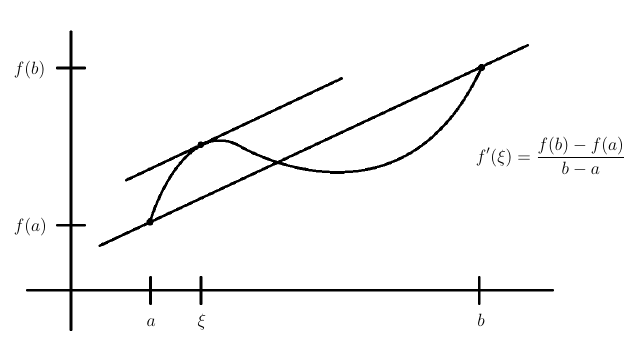
\includegraphics[width=\linewidth]{mittelwertsatz.png}
 \end{mainbox}
 
 \begin{subbox}{Cauchy - Verallgemeinerung Lagrange}
   Seien $f, g: [a, b] \to \mathbb{R}$ stetig und in $]a, b[$ differenzierbar. Dann gibt es $\xi \in ]a, b[$ mit $g'(\xi)(f(b) - f(a)) = f'(\xi)(g(b) - g(a))$. Falls $g'(x) \neq 0 \ \forall x \in ]a, b[$ folgt $g(a) \neq g(b)$ und $\frac{f(b)-f(a)}{g(b)-g(a)} = \frac{f'(\xi)}{g'(\xi)}$.
 \end{subbox}

 \begin{mainbox}{Gleichmässige Konvergenz}
  Die Folge $(f_n)$ konvergiert gleichmässig in $D$ gegen $f$ falls gilt $\forall \epsilon > 0 \ \exists N \ge 1$, so dass $\forall n \ge N, \ \forall x \in D: | f_n(x) - f(x) | < \epsilon$. \\
  Die Funktionenfolge $(g_n)$ ist gleichmässig konvergent, falls für alle $x\in D$ der Grenzwert $\limn g_n(x) = g(x)$ existiert und die Folge $(g_n)$ gleichmässig gegen $g$ konvergiert. $N$ hängt nicht von $x$ ab.
 \end{mainbox}
 
 Die Funktionenfolge $(f_n)_{n \geq 0}$ konvergiert gleichmässig gegen eine Funktion $f: D \rightarrow \mathbb{R}$ falls $\lim_{n \rightarrow \infty} \sup_{x \in D} |f_n(x) - f(x)| = 0$.\\
 
 Gleichmässige Konvergenz bewahrt Stetigkeit und Beschränktheit.
 
\subsection{Stirling'sche Formel}
Die Stirling'sche Formel ist eine Abschätzung der Fakultät. Mit der Euler-McLaurin-Formel kombiniert folgt
$$n! = \frac{\sqrt{2\pi n} \cdot n^n}{e^n} \cdot \exp(\frac{1}{12n}+R_3(n))$$
wobei $|R_3(n)| \le \frac{\sqrt{3}}{216}\cdot\frac{1}{n^2} \ \forall n \ge 1$

\begin{subbox}{Leibnizkriterium}
  Wenn $a_n \ge 0, \ \forall n \ge 1$ monoton fallend (ab gewissen $n_0$) ist und $\limn a_n = 0$ gilt, dann konvergiert $S = \sumk (-1)^{k+1} a_k$ und $a_1 - a_2 \le S \le a_1$.
  \end{subbox}
  
  \begin{mainbox}{Quotientenkriterium}
  Sei $(a_n)$ eine Folge mit $a_n \ne 0, \forall n \ge 1$. \\ Falls $\limn \sup \frac{|a_{n+1}|}{|a_n|} < 1 \implies \sum_{n=1}^\infty a_n$ konvergiert absolut. \\Falls $\limn \inf \frac{|a_{n+1}|}{|a_n|} > 1 \implies \sum_{n=1}^\infty a_n$ divergiert.  
  \end{mainbox}
  
  \begin{mainbox}{Wurzelkriterium}
  Sei $(a_n)$ eine Folge mit $a_n \ne 0, \forall n \ge 1$. Sei $q = \limn \sup \sqrt[n]{|a_n|}$. 
  \begin{itemize}
   \item $q < 1 \implies \sum_{n=1}^\infty a_n$ konvergiert absolut.
   \item $q = 1 \implies$ keine Aussage.
   \item $q > 1 \implies \sum_{n=1}^\infty a_n$ und $\sum_{n=1}^\infty |a_n|$ divergieren.
  \end{itemize}
\end{mainbox}

\subsection{Extrema in 1D}

Sei $x_0$ ein kritischer Punkt. Falls $f''(x_0) > 0$ ist $x_0$ ein Minimum, falls $f''(x_0) < 0$ ist $x_0$ ein Maximum. Ist $f''(x_0) = 0$, leiten wir ab bis $f^{(k)}(x_0) \neq 0$. Ist $f^{(k)}(x_0) > 0$ für $k$ gerade, so ist $x_0$ ein Minimum, ist $f^{(k)}(x_0) < 0$ für $k$ gerade, so ist $x_0$ ein Maximum. Ist $k$ ungerade, so ist $x_0$ ein Sattelpunkt.

\subsection{Potenzreihen}
\begin{align*}
\exp(x) &= \sumn \frac{x^n}{n!} = 1 + x + \frac{x^2}{2!} + \frac{x^3}{3!} + \cdots & r &= \infty \\
\sin(x) &= \sumn (-1)^n \frac{x^{2n + 1}}{(2n + 1)!} = x - \frac{x^3}{3!} + \frac{x^5}{5!} - \cdots & r &= \infty \\
\cos(x) &= \sumn (-1)^n \frac{x^{2n}}{(2n)!} = 1 - \frac{x^2}{2!} + \frac{x^4}{4!} - \cdots & r &= \infty \\
\ln(x + 1) &= \sumk (-1)^{k+1} \frac{x^k}{k} = x - \frac{x^2}{2} + \frac{x^3}{3} - \cdots & r &= 1 \\
\sinh(x) &= \sumn \frac{x^{2n+1}}{(2n+1)!} = x + \frac{x^3}{3!} + \frac{x^5}{5!} + \cdots & r &= \infty \\
\cosh(x) &= \sumn \frac{x^{2n}}{(2n)!} = 1 + \frac{x^2}{2!} + \frac{x^4}{4!} + \cdots & r &= \infty \\
\arctan(x) &= \sumn (-1)^n \frac{x^{2n+1}}{2n+1} = x - \frac{x^3}{3} + \frac{x^5}{5} - \cdots =  & r &= 1 \\
e^{-x} &= \sumn (-1)^n \cdot \frac{x^n}{n!} = 1 - x + \frac{x^2}{2!} - \frac{x^3}{3!} + \cdots & r &= \infty \\
\sqrt{1+x} &= 1 + \frac{x}{2} - \frac{x^2}{8} + \frac{x^3}{16} + \mathcal{O}(x^4) & r &< 1 \\
\end{align*}

\begin{mainbox}{Partialbruchzerlegung}
  Seien $p(x), q(x)$ zwei Polynome. $\int \frac{p(x)}{q(x)}$ wird wie folgend berechnet:
  \begin{enumerate}
   \item Falls $\deg(p) \ge \deg(q)$, führe eine Polynomdivision durch. Dies führt zum Integral $\int a(x) + \frac{r(x)}{q(x)}$.
   \item Berechne die Nullstellen von $q(x)$.
   \item Pro Nullstelle: Einen Partialbruch erstellen.
   \begin{itemize}[left=0pt]
    \item Einfach, reell: $x_1 \to \frac{A}{x - x_1}$
    \item $n$-fach, reell: $x_1 \to \frac{A_1}{x - x_1} + \ldots + \frac{A_r}{(x-x_1)^r}$ 
    \item Einfach, komplex: $x^2 + px + q \to \frac{Ax + B} {x^2 + px + q}$
    \item $n$-fach, komplex: $x^2 + px + q \to \frac{A_1x+b_1}{x^2+px+q} + \ldots$
   \end{itemize}
   \item Parameter $A_1, \ldots, A_n$ (bzw. $B_1, \ldots, B_n$) bestimmen. ($x$ jeweils gleich Nullstelle setzen, umformen und lösen).
 
  \end{enumerate}
 \end{mainbox}

Für ein monisches Polynom $x^n + a_{n-1} x^{n-1} + \cdots + a_0 = 0$ muss jede Nullstelle $a_0$ teilen.\\

Häufig verwendete Partialbruchzerlegungen sind bspw. $\frac{1}{q(q+1)} = \frac{1}{q} - \frac{1}{q + 1}$ oder $\frac{1}{q(q-1)(q+1)} = \frac{-1}{q} + \frac{1}{2(q+1)} + \frac{1}{2(q-1)}$.

\section{Parameterisierungen}

\begin{itemize}
  \item Kreis mit Radius $r$:{
    \begin{align*} 
      & x^2 + y^2 = r^2 & \gamma(t) = \begin{pmatrix} r \cos(t) \\ r \sin(t) \end{pmatrix}, t \in [0, 2\pi] &
    \end{align*}
  }
  \item Ellipse mit Halbachsen $a, b$:{
    \begin{align*} 
      & \frac{x^2}{a^2} + \frac{y^2}{b^2} = 1 & \gamma(t) = \begin{pmatrix} a \cos(t) \\ b \sin(t) \end{pmatrix}, t \in [0, 2\pi] &
    \end{align*}
  }
\end{itemize}

\section{Trigonometrie}

\subsection{Regeln}

\subsubsection{Doppelwinkel}
\begin{itemize}
 \item $\sin(2\alpha) = 2 \sin(\alpha) \cos(\alpha)$
 \item $\cos(2\alpha) = \cos^2(\alpha) - \sin^2(\alpha) = 1 - 2 \sin^2(\alpha)$
 \item $\tan(2\alpha) = \frac{2\tan(\alpha)}{1 - \tan^2(\alpha)}$
\end{itemize}

\subsubsection{Addition}
\begin{itemize}
 \item $\sin(\alpha + \beta) = \sin(\alpha) \cos(\beta) + \cos(\alpha) \sin(\beta)$
 \item $\cos(\alpha + \beta) = \cos(\alpha) \cos(\beta) - \sin(\alpha) \sin(\beta)$
 \item $\tan(\alpha + \beta) = \frac{\tan(\alpha) + \tan(\beta)}{1 - \tan(\alpha) \tan(\beta)}$
\end{itemize}

\subsubsection{Subtraktion}
\begin{itemize}
 \item $\sin(\alpha - \beta) = \sin(\alpha) \cos(\beta) - \cos(\alpha)\sin(\beta)$
 \item $\cos(\alpha - \beta) = \cos(\alpha) \cos(\beta) + \sin(\alpha)\sin(\beta)$
 \item $\tan(\alpha - \beta) = \frac{\tan(\alpha) - \tan(\beta)}{1+\tan(\alpha) \tan(\beta)}$
\end{itemize}

\subsubsection{Multiplikation}
\begin{itemize}
 \item $\sin(\alpha) \sin(\beta) = -\frac{\cos(\alpha + \beta) - \cos(\alpha - \beta)}{2}$
 \item $\cos(\alpha) \cos(\beta) =  \frac{\cos(\alpha + \beta) + \cos(\alpha - \beta)}{2}$
 \item $\sin(\alpha) \cos(\beta) =  \frac{\sin(\alpha + \beta) + \sin(\alpha - \beta)}{2}$
\end{itemize}

\subsubsection{Potenzen}
\begin{itemize}
 \item $\sin^2(\alpha) = \frac{1}{2}(1-\cos(2\alpha))$
 \item $\cos^2(\alpha) = \frac{1}{2}(1+\cos(2\alpha))$
 \item $\tan^2(\alpha) = \frac{1-\cos(2\alpha)}{1+\cos(2\alpha)}$
\end{itemize}

\subsubsection{Diverse}

\begin{itemize}
 \item $\sin^2(\alpha) + \cos^2(\alpha) = 1$
 \item $\cosh^2(\alpha) - \sinh^2(\alpha) = 1$
 \item $\sin(z) = \frac{e^{iz} - e^{-iz}}{2i}$ und $\cos(z) = \frac{e^{iz} + e^{-iz}}{2}$
\end{itemize}

% start larger spacing in tables
\begingroup
\renewcommand*{\arraystretch}{2}

\begin{center}
  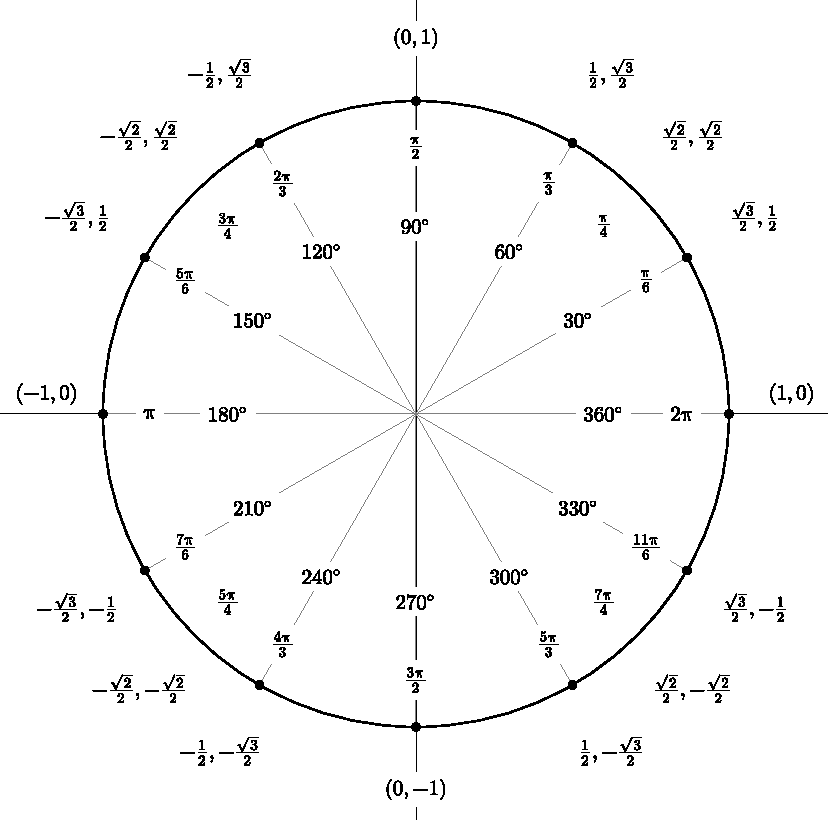
\includegraphics[width=0.7 \linewidth]{include_degrees_circle.pdf}
\end{center}

\begin{mainbox}{Wichtige Werte}
  \begin{center} 
    \begin{tabular}{c|cccccc}
      deg & 0° & 30° & 45° & 60° & 90° & 180° \\
      \midrule
      rad & 0 & $\frac{\pi}{6}$ & $\frac{\pi}{4}$ & $\frac{\pi}{3}$ & $\frac{\pi}{2}$ & $\pi$ \\
      cos & 1 & $\frac{\sqrt{3}}{2}$ & $\frac{\sqrt{2}}{2}$ & $\frac{1}{2}$ & 0 & -1 \\
      sin & 0 & $\frac{1}{2}$ & $\frac{\sqrt{2}}{2}$ & $\frac{\sqrt{3}}{2}$ & 1 & 0 \\
      tan & 0 & $\frac{1}{\sqrt{3}}$ & 1 & $\sqrt{3}$ & $+\infty$ & 0 \\
    \end{tabular}
  \end{center}
\end{mainbox}

\section{Tabellen}

\subsection{$n$-te Ableitungen}
\begin{center}
  \begin{tabularx}{\linewidth}{>{\centering\arraybackslash}X>{\centering\arraybackslash}X}
  \toprule
  $\mathbf{f(x)}$ & $\mathbf{f^{(n)}(x)}$ \\
  \midrule
  $\sin(x)$ & $\sin(\frac{n\pi}{2} + x)$\\
  $f + g$ & $f^{(n)} + g^{(n)}$\\
  $f \cdot g$ & $\sum\limits_{k=0}^{n}\binom{n}{k}f^{(k)}g^{(n-k)}$\\
  \bottomrule
  \end{tabularx}
\end{center}

\subsection{Trigonometrische Identitäten}
\begin{center}
 \begin{tabularx}{\linewidth}{>{\centering\arraybackslash}X>{\centering\arraybackslash}X}
  \toprule
  $\mathbf{f(x)}$ & $\mathbf{f(x)}$ \\
  \midrule
  $\sin(\arccos (x))$ & $\sqrt{1-x^2}$\\
  $\cos(\arcsin(x))$ & $\sqrt{1-x^2}$\\
  $\sin(\arctan(x))$ & $\frac{x}{\sqrt{1+x^2}}$\\
  $\cos(\arctan(x))$ & $\frac{1}{\sqrt{1+x^2}}$\\
  $\tan(\arcsin(x))$ & $\frac{x}{\sqrt{1-x^2}}$\\
  $\tan(\arccos(x))$ & $\frac{\sqrt{1-x^2}}{x}$\\
  \bottomrule
 \end{tabularx}
\end{center}

\subsection{Grenzwerte}
\begin{center}
  \begin{tabularx}{\linewidth}{XX}
    \toprule
    $\limxi \frac{1}{x} = 0$ & $\limxi 1 + \frac{1}{x} = 1$ \\
    $\limxi e^x = \infty$ & $\limxn e^x = 0$ \\
    $\limxi e^{-x} = 0$ & $\limxn e^{-x} = \infty$ \\
    $\limxi \frac{e^x}{x^m} = \infty$ & $\limxn xe^x = 0$ \\
    $\limxi \ln(x) = \infty$ & $\limxo \ln(x) = -\infty$ \\
    $\limxi (1+x)^{\frac{1}{x}} = 1$ & $\limxo (1+x)^{\frac{1}{x}} = e$ \\
    $\limxi (1+\frac{1}{x})^b = 1$ & $\limxi n^{\frac{1}{n}} = 1$ \\
    $\lim_{x\to\pm\infty} (1 + \frac{1}{x})^x = e$ & $\limxi (1-\frac{1}{x})^x = \frac{1}{e}$ \\
    $\lim_{x\to\pm\infty} (1 + \frac{k}{x})^{mx} = e^{km}$ & $\limxi (\frac{x}{x+k})^x = e^{-k}$ \\
    $\limxo \frac{a^x -1}{x} = \ln(a), \newline \forall a > 0$ &
    $\limxi x^a q^x = 0, \newline \forall 0 \le q < 1$ \\
  \end{tabularx}
  \begin{tabularx}{\linewidth}{XX}
    $\limxo \frac{\sin x}{x} = 1$ & $\limxo \frac{\sin kx}{x} = k$\\
    $\limxo \frac{1}{\cos x} = 1$ & $\limxo \frac{\cos x -1}{x} = 0$ \\
    $\limxo x \sin(\frac{1}{x}) = 0$ & $\limxo x \log x = 0$\\
    $\limxo \frac{1 - \cos x}{x^2} = \frac{1}{2}$ & $\limxo \frac{e^x-1}{x} = 1$ \\
    $\limxo \frac{x}{\arctan x} = 1$ & $\limxi \arctan x = \frac{\pi}{2}$ \\
    $\limxo \frac{e^{ax}-1}{x} = a$ & $\limxo \frac{\ln(x+1)}{x} = 1$ \\
    $\lim_{x\to 1} \frac{\ln(x)}{x-1} = 1$ & $\limxi \sqrt{x^2 + c} - x = 0$ \\
    $\limxi \sqrt[x]{x} = 1$ & $\limxi x(\sqrt[x]{n} - 1) = \ln(n)$ \\
    \bottomrule
  \end{tabularx}
\end{center}

\subsection{Rekursive Integrale}

$J_n = \int \frac{1}{(1 + x^2)^n} \dx$, dann $J_{n+1} = \frac{x}{2n(1 + x^2)^n} + (\frac{2n - 1}{2n})J_n$ mit $J_1 = \arctan(x)$.

\subsection{Binomischer Lehrsatz}

$$(x+y)^n = \sum_{k=0}^n {n \choose k} x^{n-k} y^k$$

\subsection{Ableitungen (I)}
\begin{center}
  % the c>{\centering\arraybackslash}X is a workaround to have a column fill up all space and still be centered
  \begin{tabularx}{\linewidth}{c>{\centering\arraybackslash}Xc}
  \toprule
  $\mathbf{F(x)}$ & $\mathbf{f(x)}$ & $\mathbf{f'(x)}$ \\
  \midrule
  $\frac{x^{-a+1}}{-a+1}$ & $\frac{1}{x^a}$ & $\frac{a}{x^{a+1}}$ \\
  $\frac{x^{a+1}}{a+1}$ & $x^a \ (a \ne -1)$ & $a \cdot x^{a-1}$ \\
  $\frac{1}{k \ln(a)}a^{kx}$ & $a^{kx}$ & $ka^{kx} \ln(a)$ \\
  $\ln |x|$ & $\frac{1}{x}$ & $-\frac{1}{x^2}$ \\
  $\frac{2}{3}x^{3/2}$ & $\sqrt{x}$ & $\frac{1}{2\sqrt{x}}$\\
  $-\cos(x)$ & $\sin(x)$ & $\cos(x)$ \\
  $\sin(x)$ & $\cos(x)$ & $-\sin(x)$ \\
  $\frac{1}{2}(x-\frac{1}{2}\sin(2x))$ & $\sin^2(x)$ & $2 \sin(x)\cos(x)$ \\
  $\frac{1}{2}(x + \frac{1}{2}\sin(2x))$ & $\cos^2(x)$ & $-2\sin(x)\cos(x)$ \\
  $-\ln|\cos(x)|$ & $\tan(x)$ & $\frac{1}{\cos^2(x)} = 1 + \tan^2(x)$  \\
  $\cosh(x)$ & $\sinh(x)$ & $\cosh(x)$ \\
  $\log(\cosh(x))$ & $\tanh(x)$ & $\frac{1}{\cosh^2(x)} = 1 - \tanh^2(x)$ \\
  $\ln | \sin(x)|$ & $\cot(x)$ & $-\frac{1}{\sin^2(x)}$ \\
  $\frac{1}{c} \cdot e^{cx}$ & $e^{cx}$ & $c \cdot e^{cx}$ \\
  $x(\ln |x| - 1)$ & $\ln |x|$ & $\frac{1}{x}$ \\
  $\frac{1}{2}(\ln(x))^2$ & $\frac{\ln(x)}{x}$ & $\frac{1 - \ln(x)}{x^2}$ \\
  $\frac{x}{\ln(a)} (\ln|x| -1)$ & $\log_a |x|$ & $\frac{1}{\ln(a)x}$ \\
  \bottomrule
  \end{tabularx}
\end{center}


\subsection{Ungleichungen}
\begin{center}
  \begin{tabularx}{\linewidth}{>{\centering\arraybackslash}X>{\centering\arraybackslash}X}
    $(1+x)^n \geq 1+ n\cdot x$ \, $\forall n\in \mathbb{N}, x > -1$\\
    $e^x \geq 1 + x$ \, $\forall x\in \mathbb{R}$\\
    $2|xy| \leq \epsilon x^2 + \frac{1}{\epsilon} y^2$ für $\forall \epsilon > 0$ und $\forall x,y \in \mathbb{R}$\\
    $|\langle x,y \rangle| \leq ||x|| \cdot ||y||$ für $\forall x,y, \in \mathbb{R}^n$\\
    $\sqrt[n]{x_1 x_2 \cdots x_n} \leq \frac{x_1 + x_2 + \cdots + x_n}{n}$
  \end{tabularx}
\end{center}

\subsection{Weitere Integrale}
\begin{center}
 \begin{tabularx}{\linewidth}{>{\centering\arraybackslash}X>{\centering\arraybackslash}X}
  \toprule
  $\mathbf{f(x)}$ & $\mathbf{F(x)}$ \\
  \midrule
  $\int f'(x) f(x) \dx$ & $\frac{1}{2}(f(x))^2$ \\
  $\int \frac{f'(x)}{f(x)} \dx$ & $\ln|f(x)|$ \\
  $\int_{-\infty}^\infty e^{-x^2} \dx$ & $\sqrt{\pi}$ \\
  $\int (ax+b)^n \dx$ & $\frac{1}{a(n+1)}(ax+b)^{n+1}$ \\
  $\int x(ax+b)^n \dx$ & $\frac{(ax+b)^{n+2}}{(n+2)a^2} - \frac{b(ax+b)^{n+1}}{(n+1)a^2}$ \\
  $\int (ax^p+b)^n x^{p-1} \dx$ & $\frac{(ax^p+b)^{n+1}}{ap(n+1)}$ \\
  $\int (ax^p + b)^{-1} x^{p-1} \dx$ & $\frac{1}{ap} \ln |ax^p + b|$ \\
  $\int \frac{ax+b}{cx+d} \dx$ & $\frac{ax}{c} - \frac{ad-bc}{c^2} \ln |cx +d|$ \\
  $\int \frac{1}{x^2+a^2} \dx$ & $\frac{1}{a} \arctan \frac{x}{a}$ \\
  $\int \frac{1}{x^2 - a^2} \dx$ & $\frac{1}{2a} \ln\left| \frac{x-a}{x+a} \right|$ \\
  $\int \sqrt{a^2 - x^2} \dx $ & $\frac{a^2}{2} \arcsin(\frac{x}{a}) + \frac{x}{2} \sqrt{a^2 - x^2}$ \\
  $\int \csc(x) \dx $ & $\ln|\csc(x) + \cot(x)|$ \\
  $\int \sec(x) \dx $ & $\ln|\sec(x) + \tan(x)|$ \\
  $\int \cot(x) \dx $ & $\ln|\sin(x)|$ \\
  \bottomrule
 \end{tabularx} 
\end{center}

\subsection{Ableitungen (II)}
\begin{center}
  % the c>{\centering\arraybackslash}X is a workaround to have a column fill up all space and still be centered
  \begin{tabularx}{\linewidth}{c>{\centering\arraybackslash}Xc}
  \toprule
  $\mathbf{F(x)}$ & $\mathbf{f(x)}$ & $\mathbf{f'(x)}$ \\
  \midrule
  $\frac{1}{2}(\cosh(x)\sinh(x)+1)$ & $\cosh(x)^2$ & $2\sinh(x)\cosh(x)$\\
  $\frac{1}{2}(\sinh(x)\cosh(x) + x)$ & $\sinh(x)^2$ & $2\sinh(x)\cosh(x)$\\
  \bottomrule
  \end{tabularx}
\end{center}

\subsection{Weitere Ableitungen}
\begin{center}
  \begin{tabularx}{\linewidth}{>{\centering\arraybackslash}X>{\centering\arraybackslash}X}
  \toprule
  $\mathbf{F(x)}$ & $\mathbf{f(x)}$ \\
  \midrule
  $\arcsin(x)$ & $\frac{1}{\sqrt{1 - x^2}}$ \\
  $\arccos(x)$ & $\frac{-1}{\sqrt{1 - x^2}}$ \\
  $\arctan(x)$ & $\frac{1}{1 + x^2}$ \\ 
  $\text{arsinh}(x)$ & $\frac{1}{\sqrt{1 + x^2}}$ \\
  $\text{arcosh}(x)$ & $\frac{1}{\sqrt{x^2 - 1}}$ \\
  $\text{artanh}(x)$ & $\frac{1}{1 - x^2}$ \\
  $\text{arccot}(x)$ & $-\frac{1}{1 + x^2}$ \\
  $x^x \ (x > 0)$ & $x^x \cdot (1 + \ln x)$ \\
  $\cosh(x)$ & $\sinh(x)$ \\
  $\sinh(x)$ & $\cosh(x)$ \\
  \bottomrule
  \end{tabularx}
\end{center}

\subsection{Uneigentliche Integrale}
$$\int_1^\infty \frac{1}{x^\alpha} \dx = \begin{cases}
  \text{divergiert, } & \alpha \leq 1\\
  \frac{1}{\alpha - 1} & \alpha > 1
\end{cases}$$
$$\int_0^1 \frac{1}{x^\alpha} \dx = \begin{cases}
  \text{divergiert, } & \alpha \geq 1\\
  \frac{1}{1- \alpha} & \alpha < 1
\end{cases}$$
$$\int_0^\infty e^{-x} \dx = 1$$
$$\int_0^\infty e^{-x}x^{s-1} \dx = \begin{cases}
  \text{divergiert, } & s \leq 0\\
  (s-1)! & s > 0
\end{cases}$$
$$\int_0^\infty \sin(x^2) \dx = \sqrt{\frac{\pi}{8}}$$

\subsection{Gerade und ungerade Funktionen}
\begin{itemize}
  \item Die Verknüpfung von ungeraden Funktionen ist ungerade. 
  \item Sei $g$ gerade und $f$ beliebig. $f \circ g$ ist gerade.
  \item Sei $f$ gerade und $g$ ungerade. $g \circ f$ und $f \circ g$ sind gerade.
  \item Produkt einer geraden und einer ungeraden Funktion ist ungerade.
  \item Produkt zweier ungerader Funktionen ist gerade.
  \item Produkt zweier gerader Funktionen ist gerade.
  \item Für $f: [-a, a] \to \mathbb{R}$ stetig und ungerade, d.h. $f(-x) = -f(x)$ gilt $\int_{-a}^a f(x) \dx = 0$.
\end{itemize}

\subsection{Partielle Integration - DI Method}
Berechne $\int x^2 \cos(x) \dx = x^2 (-\frac{1}{3}\cos(3x)) - 2x(-\frac{1}{9}\sin(3x)) + 2\frac{1}{27}\cos(3x) - \int 0 \cdot \frac{1}{27} \cos(3x) \dx$.

Multipliziere Diagonal wie im Beispiel.

\begin{table}[h]
  \begin{tabular}{lll}
    & D & I \\
  + & $x^2$ & $\sin(3x)$  \\
  - & $2x$ & $-\frac{1}{3}\cos(3x)$  \\
  + & $2$ & $-\frac{1}{9}\sin(3x)$  \\
  - & $0$ & $\frac{1}{27}\cos(3x)$  
  \end{tabular}
\end{table}

Aufhören falls:
\begin{itemize}
  \item $0$ in D-Spalte.
  \item Produkt einer Reihe einfach integrierbar. Addiere oder subtrahiere je nach Reihe das Integral des Produkts.
  \item Eine Reihe wiederholt sich. Verwende Rekurrenz.
\end{itemize}

\subsection{Synthetische Division}
Berechne $\frac{6x^3 + 5x^2 - 7}{3x^2 - 2x - 1} = 2x + 3 + \frac{8x - 4}{3x^2 -2x - 1}$:\\
\begin{center}
  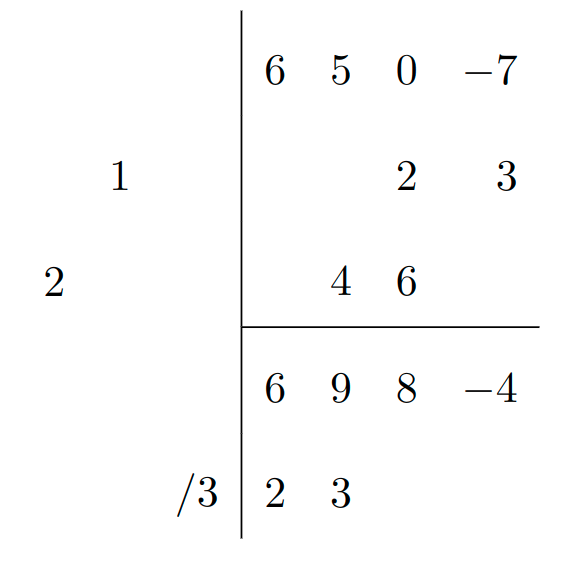
\includegraphics[width=0.4 \linewidth]{synthetic-division.png}
\end{center}

% end of larger array spacing
\endgroup
\end{document}
